% ======================================================================
\subsection{Exclusive CKM-suppressed decays}
\label{slbdecays_b2uexcl}
% ----------------------------------------------
In this section, we list results on exclusive charmless semileptonic branching fractions
and determinations of $\vub$ based on $\Bb\to\pi\ell\nub$ decays.
The measurements are based on two different event selections: tagged
events, in which case the second $B$ meson in the event is fully
reconstructed in either a hadronic decay (``had. tag'') or in a 
CKM-favored semileptonic decay (``sl. tag''); and untagged events, in which case the momentum
of the undetected neutrino is inferred from measurements of the total 
momentum sum of the detected particles and the knowledge of the initial state.
We also present averages for $\Bb\to\rho\ell\nub$, $\Bb\to\omega\ell\nub$, $\Bb\to\eta\ell\nub$ and
$\Bb\to\eta'\ell\nub$.

The results for the full and partial branching fractions for $\Bb\to\pi\ell\nub$ are given
in Table~\ref{tab:pilnubf} and shown in Figure~\ref{fig:xlnu}.   

When averaging these results, systematic uncertainties due to external
inputs, e.g., form factor shapes and background estimates from the
modeling of $\Bb\to X_c\ell\nub$ and $\Bb\to X_u\ell\nub$ decays, are
treated as fully correlated (in the sense of Eq.~\ref{eq:correlrho}).
Uncertainties due to experimental reconstruction effects are treated
as fully correlated among measurements from a given experiment. Varying
the assumed dependence of the quoted errors on the measured value
for error sources where the dependence was not obvious had no significant impact.

\begin{sidewaystable}[!htb]
\begin{center}
\caption{\label{tab:pilnubf}
Summary of exclusive determinations of $\cbf(\Bb\to\pi
\ell\nub)$. The errors quoted
correspond to statistical and systematic uncertainties, respectively.
Measured branching fractions for $B\rightarrow \pi^0 l \nu$ have been
multiplied by $2\times \tau_{B^0}/\tau_{B^+}$ in accordance with
isospin symmetry. The labels ``$B_{reco}$'' and ``SL'' tags refer to
the type of $B$
decay tag used in a measurement, and ``untagged'' refers to an untagged measurement.}
\begin{small}
\begin{tabular}{|lcccc|}
\hline
& $\cbf [10^{-4}]$
& $\cbf(q^2<12\,\gev^2/c^2) [10^{-4}]$
& $\cbf(q^2<16\,\gev^2/c^2) [10^{-4}]$
& $\cbf(q^2>16\,\gev^2/c^2) [10^{-4}]$
\\
\hline\hline
CLEO $\pi^+,\pi^0$~\cite{Adam:2007pv}
& $1.38\pm 0.15\pm 0.11\ $ 
& $0.70\pm 0.12\pm 0.07$
& $0.97\pm 0.13\pm 0.09$
& $0.41\pm 0.08\pm 0.04$
\\ 
\babar $\pi^+,\pi^0$~\cite{delAmoSanchez:2010af}
& $1.41\pm 0.05\pm 0.08\ $
& $0.88\pm 0.04\pm 0.05$
& $1.10\pm 0.04\pm 0.06$
& $0.32\pm 0.02\pm 0.03$
\\  
\babar $\pi^+$~\cite{delAmoSanchez:2010zd}
& $1.42\pm 0.05\pm 0.07\ $
& $0.83\pm 0.03\pm 0.04$
& $1.09\pm 0.04\pm 0.05$
& $0.33\pm 0.03\pm 0.03$
\\  
Belle $\pi^+$~\cite{Ha:2010rf}
& $1.49\pm 0.04\pm 0.07\ $
& $0.83\pm 0.03\pm 0.04$
& $1.10\pm 0.03\pm 0.05$
& $0.40\pm 0.02\pm 0.02$
\\  
Belle SL $\pi^+$~\cite{Hokuue:2006nr}
& $1.42\pm 0.19\pm 0.15\ $
& $0.80\pm 0.14\pm 0.08$
& $1.04\pm 0.16\pm 0.11$
& $0.37\pm 0.10\pm 0.04$
\\ 
Belle SL $\pi^0$~\cite{Hokuue:2006nr}
& $1.41\pm 0.26\pm 0.15\ $
& $0.71\pm 0.17\pm 0.08$
& $1.04\pm 0.22\pm 0.12$
& $0.36\pm 0.15\pm 0.04$
\\ 
\babar SL $\pi^+$~\cite{Aubert:2008bf}
& $1.39\pm 0.21\pm 0.08\ $
& $0.77\pm 0.14\pm 0.05$
& $0.92\pm 0.16\pm 0.05$
& $0.46\pm 0.13\pm 0.03$
\\ 
\babar SL $\pi^0$~\cite{Aubert:2008bf}
& $1.78\pm 0.28\pm 0.15\ $
& $1.07\pm 0.20\pm 0.09$
& $1.34\pm 0.22\pm 0.11$
& $0.44\pm 0.17\pm 0.06$
\\ 
\babar $B_{reco}$ $\pi^+$~\cite{Aubert:2006ry}
& $1.07\pm 0.27\pm 0.19\ $
& $0.26\pm 0.15\pm 0.04$
& $0.42\pm 0.18\pm 0.06$
& $0.65\pm 0.20\pm 0.13$
\\ 
\babar $B_{reco}$ $\pi^0$~\cite{Aubert:2006ry}
& $1.52\pm 0.41 \pm0.30\ $
& $0.67\pm 0.30\pm 0.12$
& $1.04\pm 0.35\pm 0.18$
& $0.48\pm 0.22\pm 0.12$
\\ 
Belle $B_{reco}$ $\pi^+$~\cite{:2008kn}
& $1.12\pm 0.18\pm 0.05\ $
& $0.65\pm 0.14\pm 0.03$
& $0.85\pm 0.16\pm 0.04$
& $0.26\pm 0.08\pm 0.01$
\\ 
Belle $B_{reco}$ $\pi^0$~\cite{:2008kn}
& $1.22\pm 0.22\pm 0.05\ $
& $0.65\pm 0.19\pm 0.03$
& $0.80\pm 0.19\pm 0.03$
& $0.41\pm 0.11\pm 0.02$
\\  \hline
{\bf Average}
& \mathversion{bold}$1.42\pm 0.03\pm 0.04\ $
& \mathversion{bold}$0.81\pm 0.02\pm 0.03$
& \mathversion{bold}$1.05\pm 0.02\pm 0.03$
& \mathversion{bold}$0.37\pm 0.01\pm 0.02$
\\ 
\hline
\end{tabular}\\
\end{small}
\end{center}
\end{sidewaystable}


\begin{figure}[!ht]
 \begin{center}
  \unitlength1.0cm % coordinates in cm
  \begin{picture}(14.,8.0)  %ys(25.,6.)
  % \put(  8.0,  0.0){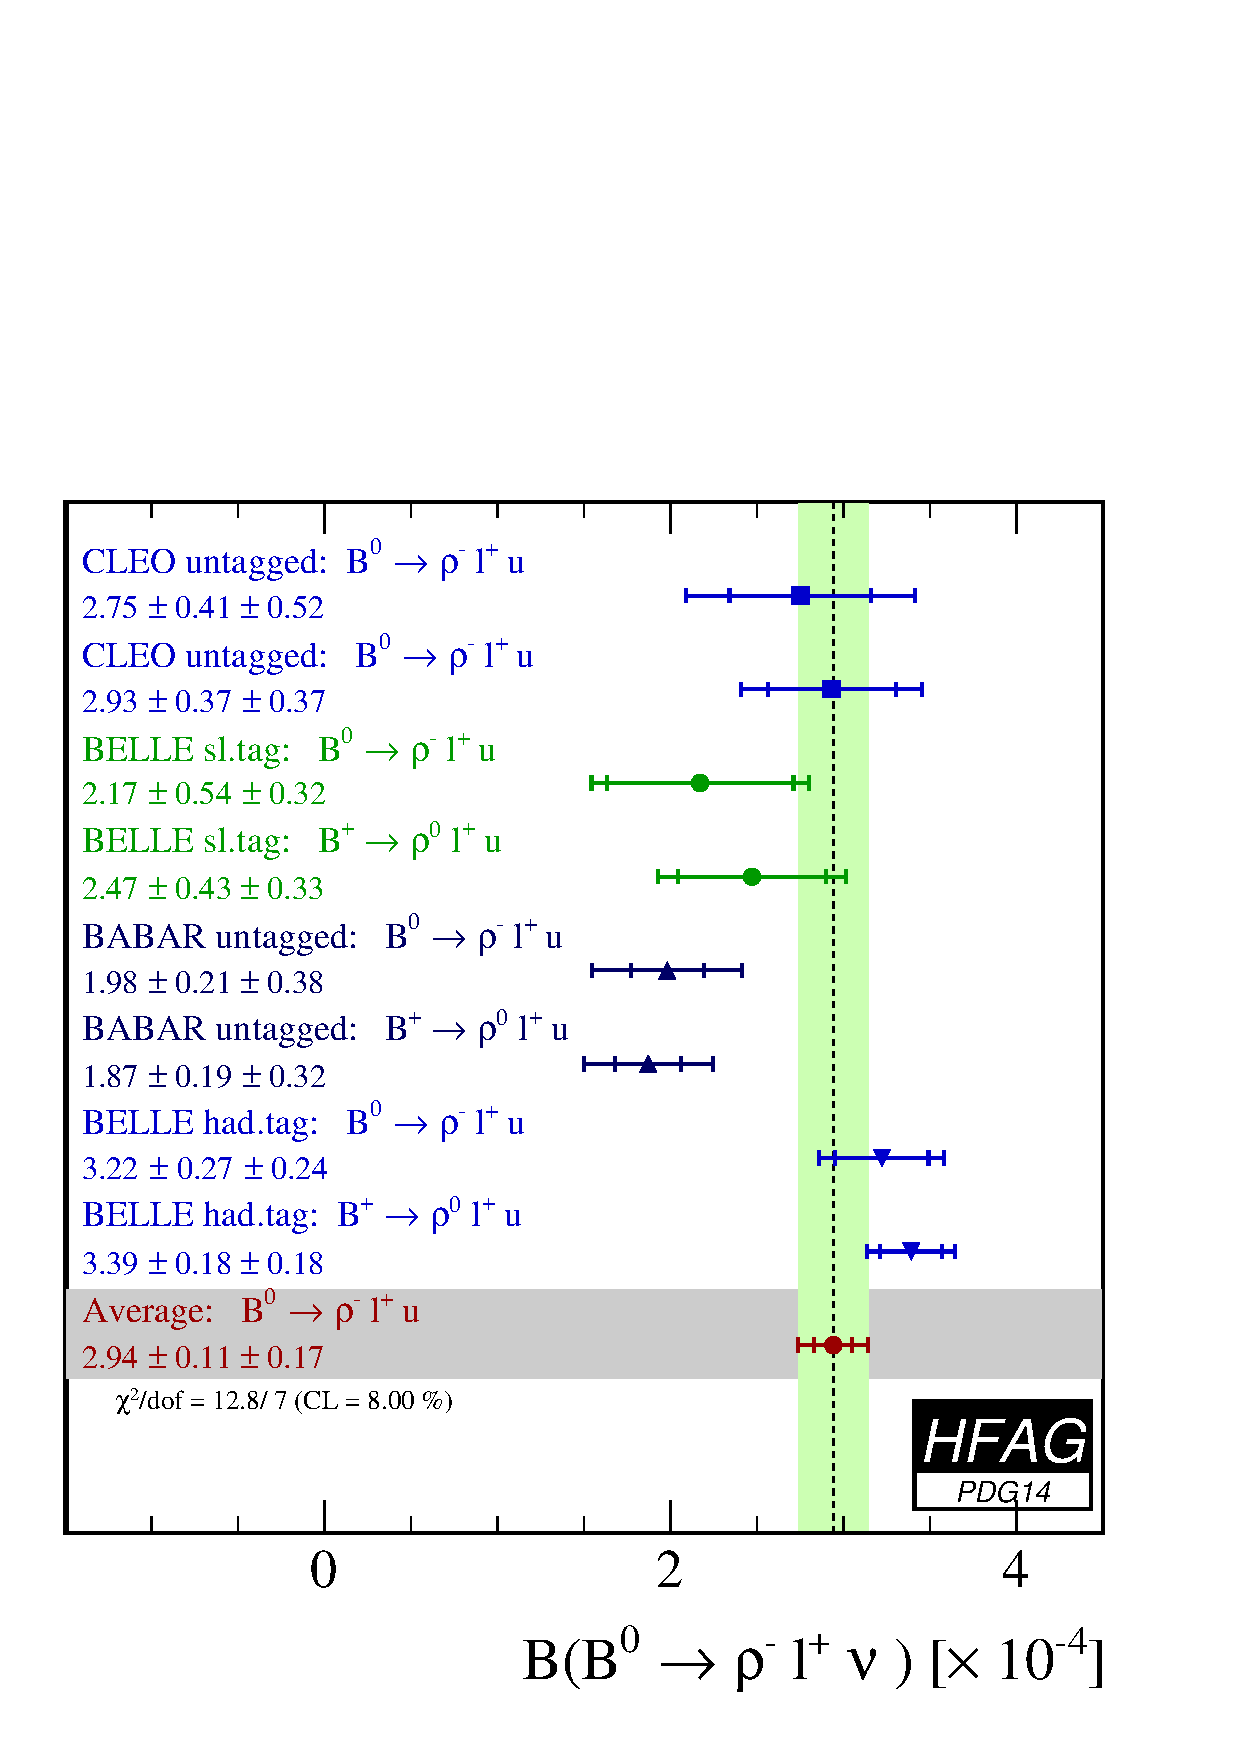
\includegraphics[width=8.0cm]{figures/slb/rholnu.pdf}}
   \put( 2.0,  0.0){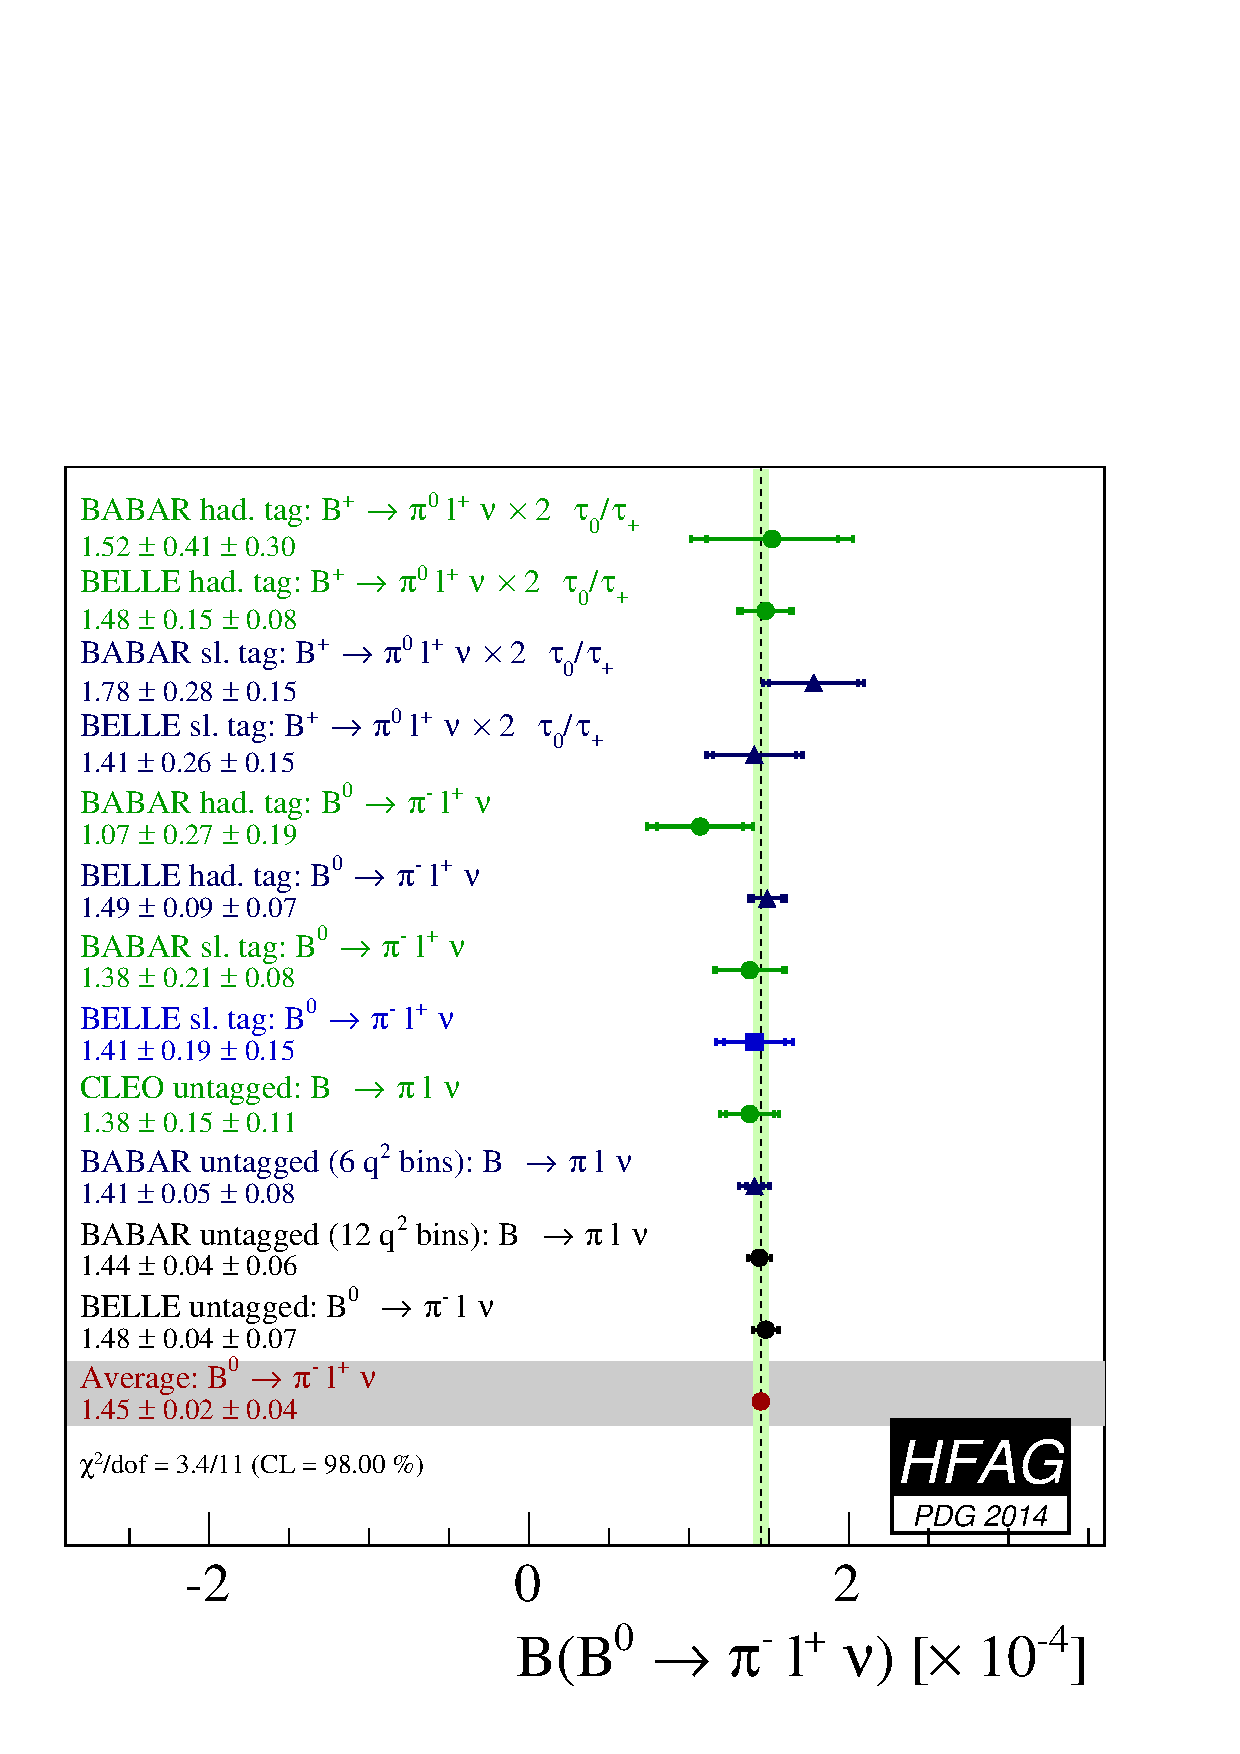
\includegraphics[width=8.8cm]{figures/slb/pilnu.pdf}
   }
 %  \put(  5.5,  7.3){{\large\bf a)}}  
 %  \put( 14.4,  7.3){{\large\bf b)}}
   \end{picture} \caption{
Summary of exclusive determinations of $\cbf(\Bb\to\pi\ell\nub)$ and their average.
Measured branching fractions for $B^+ \rightarrow \pi^0 l^+ \nu$ have been
multiplied by $2\times \tau_{B^0}/\tau_{B^+}$ in accordance with
isospin symmetry. The labels ``had. tag'' and ``sl. tag''
refer to the type of $B$ tag used in the measurement; ``untagged'' refers to an untagged measurement.
The results from the untagged measurements by CLEO and \babar are based on a combined analysis of
$B^0 \rightarrow \pi^- l^+ \nu$  and $B^+ \rightarrow \pi^0 l^+ \nu$ decays using isospin relations. 
%(b) Summary of exclusive determinations of $\cbf(\Bb\to\rho\ell\nub)$ and their average.
}
\label{fig:xlnu}
\end{center}
\end{figure}

The determination of \vub\ from $\Bb\to\pi\ell\nub$ decays is
shown in Table~\ref{tab:pilnuvub}, and uses our averages for the partial branching
fractions given in Table~\ref{tab:pilnubf}, combined with various form factor calculations. 
Two theoretical approaches are used: unquenched lattice QCD (LQCD) and QCD light-cone sum rules (LCSR).
Lattice calculations of the form factors are limited to small hadron momenta, i.e.
large $q^2$, while calculations based on light-cone sum rules are restricted
to small $q^2$. 


\begin{table}[hbtf]
\caption{\label{tab:pilnuvub}
Determinations of \vub\ based on the average partial
$\Bb\to\pi\ell\nub$ decay branching fractions stated in
Table~\ref{tab:pilnubf}. 
The $q^2$ ranges for the partial branching fractions corresponding to the 
validity ranges of the form factor calculations are indicated. 
The first uncertainty is experimental and the second is from theory.  
}
%\scriptsize
%\vspace{5mm} 
\begin{center}
\renewcommand{\arraystretch}{1.2}
\begin{tabular}{|lcc|}
\hline
Method                                         & $q^2$ range [$\gev^2/c^2$] & $\Vub [10^{-3}]$ \\\hline\hline
Khodjamirian et al. (LCSR) ~\cite{Khodjamirian:2011ub} & 0 -- 12                    & $3.41\pm 0.06 {}^{+0.37}_{-0.32}$ \\ \hline
Ball \& Zwicky (LCSR)~\cite{Ball:2004ye}              & 0 -- 16                    & $3.58\pm 0.06 {}^{+0.59}_{-0.40}$ \\ \hline
HPQCD (LQCD)~\cite{Dalgic:2006dt}                     & 16 -- 26.4                 & $3.52\pm 0.08 {}^{+0.61}_{-0.40}$ \\  \hline
FNAL/MILC (LQCD)~\cite{Bailey:2008wp}                 & 16 -- 26.4                 & $3.36\pm 0.08 {}^{+0.37}_{-0.31}$ \\ 
%APE, $q^2>16\,\gev^2/c^2$~\cite{Abada:2000ty}         & $3.72\pm 0.21 {}^{+1.43}_{-0.66}$ \\ 
\hline
\end{tabular}
\end{center}
\end{table}


An alternative method to determine \vub\ from $\Bb\to\pi\ell\nub$ decays that makes use
of the measurement over the full $q^2$ range is based on a simultaneous fit of a
$B\to \pi$ form factor parameterization to data and theory predictions. 
We choose the BCL (Bourrely, Caprini, Lellouch) parameterization~\cite{Bourrely:2008za} up to order $z^2$.
There are 3+1 fit parameters: the three coefficients of the BCL power series ($b_0$, $b_1$, $b_2$)
and \Vub, which is determined from the relative normalization between data and theory predications. 
As the shape of the $q^2$ spectrum is determined by only two parameters ($b_1$ and $b_2$), we quote
the ratios $b_1/b_0$ and $b_2/b_0$ as results for the shape determined in the fit.

The result of the simultaneous fit to the four most precise measurements from \babar and Belle 
(\babar untagged 6 $q^2$ bins, \babar untagged 12 $q^2$ bins, Belle untagged, Belle had. tag)
and the FNAL/MILC LQCD calculations is shown in Figure~\ref{fig:vub_pilnu_simultaneous}~(a). 
The fit probability is 0.053 ($\chi^2/dof = 60.2/44$) and we obtain the following values:
\begin{eqnarray}
\Vub &=& (3.28 \pm 0.29) \times 10^{-3}, \\
b_1/b_0 &=& -1.02 \pm 0.18, \\
b_2/b_0 &=& -1.20 \pm 0.57.
\end{eqnarray}
The fit results correspond to a value of the product $f_+(0)\Vub$ of $(0.923 \pm 0.024) \times 10^{-3}$. 
The correlation matrix of the fit parameters is:
\begin{center}
\begin{tabular}{ccccc}
      & $b_0$ & $b_1$ & $b_2$ & \Vub  \\
$b_0$ & 1.00  & -0.54 &  0.15 & -0.29 \\
$b_1$ &       &  1.00 & -0.89 &  0.24 \\ 
$b_2$ &       &       &  1.00 & -0.14 \\  
\Vub  &       &       &       &  1.00 \\
\end{tabular}
\end{center}

\begin{figure}[!ht]
 \begin{center}
  \unitlength1.0cm % coordinates in cm

  \begin{picture}(14.,8.0)  %ys(25.,6.)
   \put( -0.5,  0.0){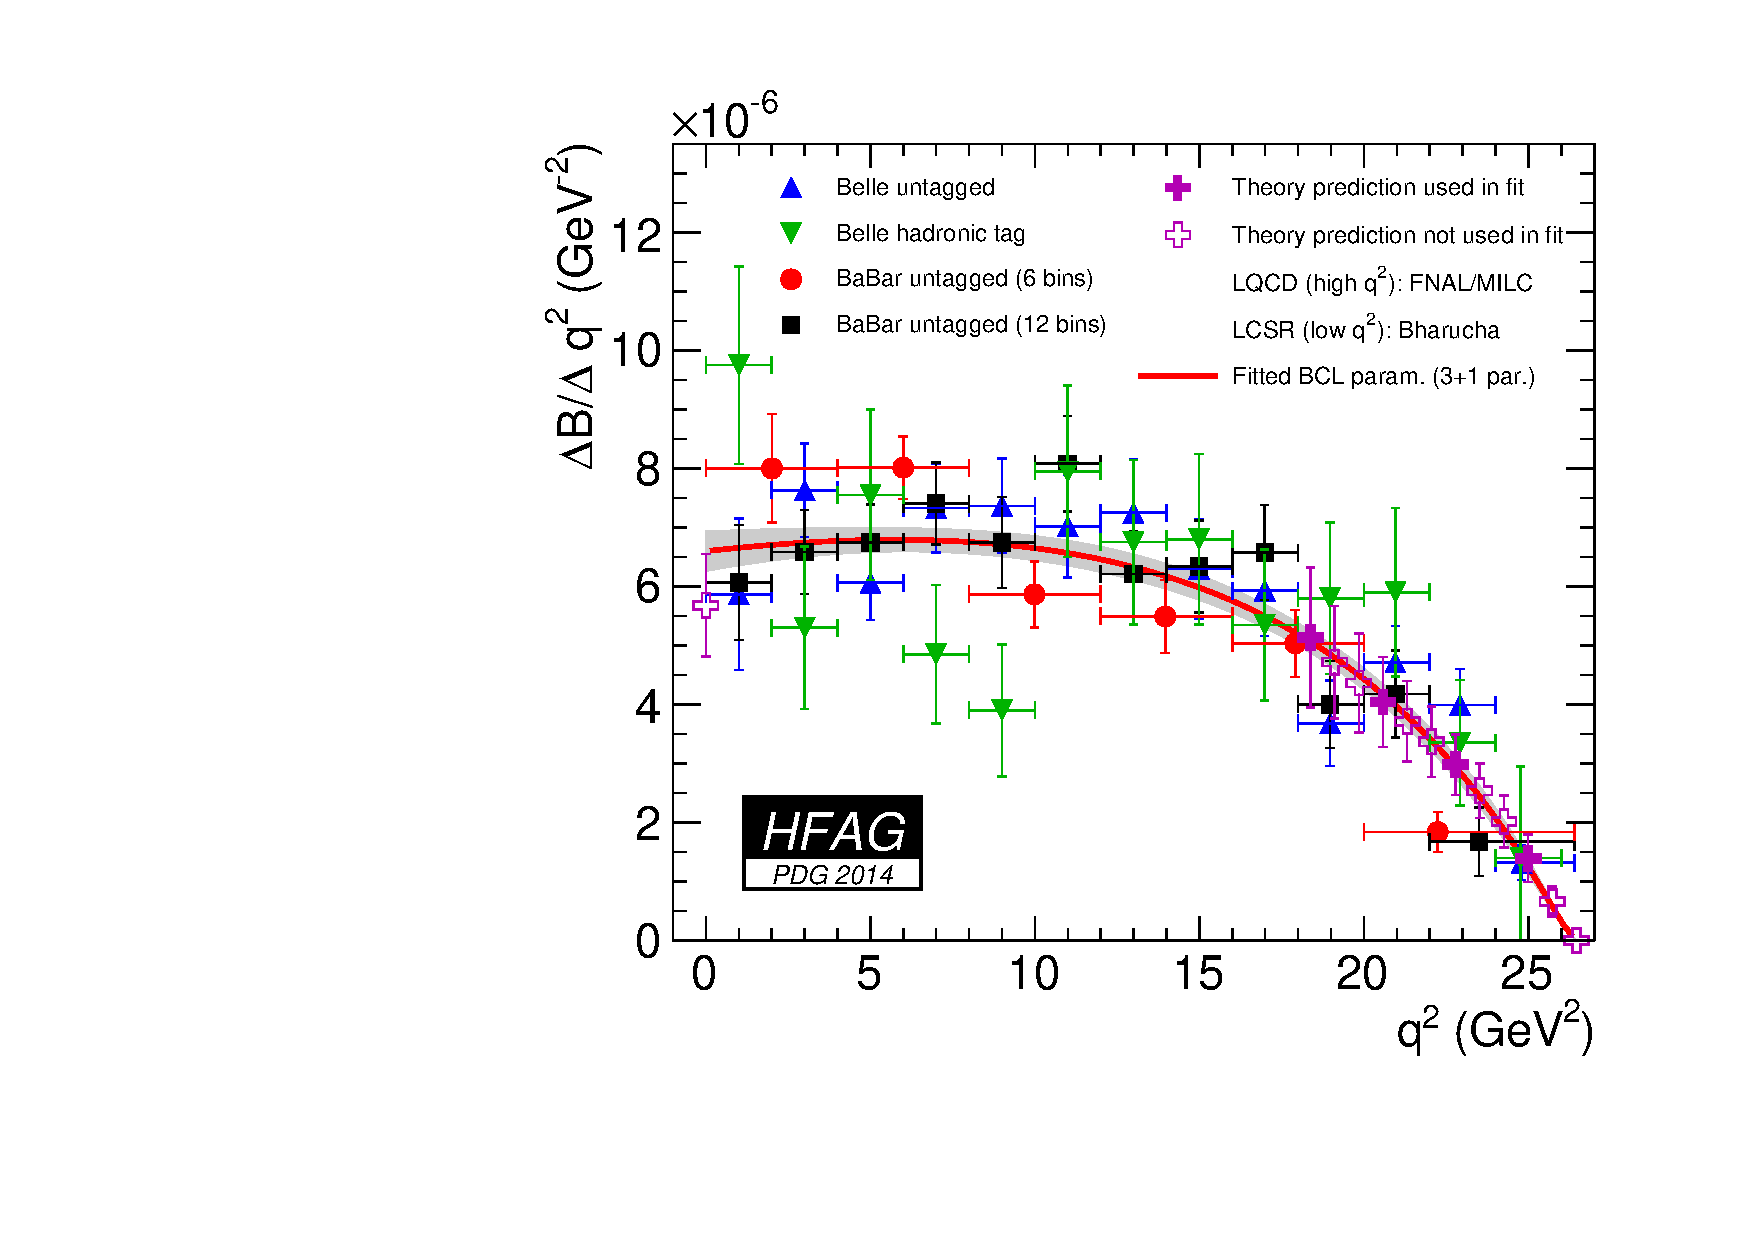
\includegraphics[width=8.0cm]{figures/slb/vub_pilnu_combinedFit_FNAL.pdf}}
   \put( 8.0,  0.0){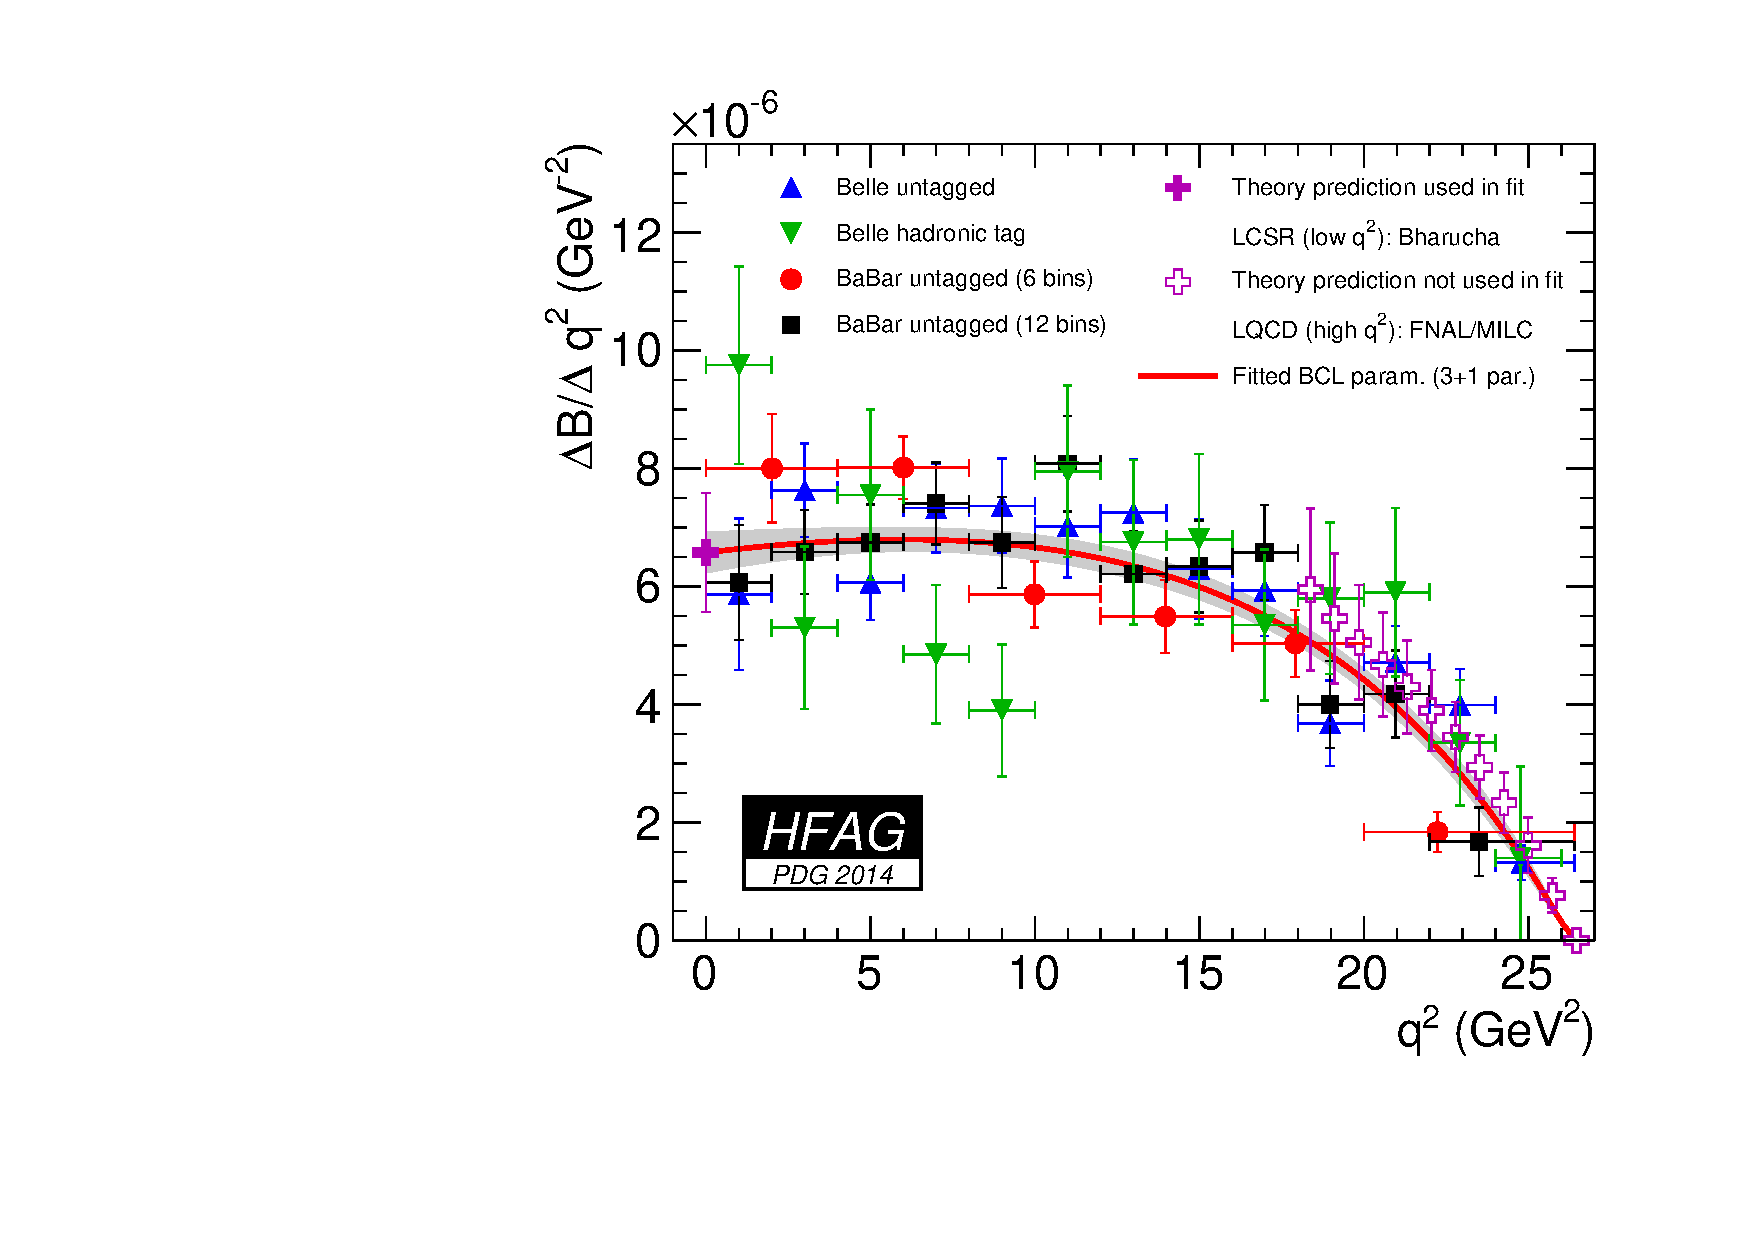
\includegraphics[width=8.0cm]{figures/slb/vub_pilnu_combinedFit_LCSR.pdf}} 
   \put(  5.8,  3.6){{\large\bf a)}}     
   \put( 14.3,  3.6){{\large\bf b)}}
   \end{picture} 
   \caption{
    Simultaneous fit of the BCL parameterization with 3+1 parameters to \babar and Belle $\Bb\to\pi\ell\nub$ data
    and the theory prediction from (a) FNAL/MILC LQCD calculations~\cite{Bailey:2008wp} 
    (yielding $\Vub = (3.28 \pm 0.29) \times 10^{-3}$)
    and (b) LCSR~\cite{Bharucha:2012wy} at $q^2=0$ (yielding $\Vub = (3.53 \pm 0.29) \times 10^{-3}$).}
\label{fig:vub_pilnu_simultaneous}
\end{center}
\end{figure}

The simultaneous fit has also been performed using the most recent result for $f_+(0)$ from LCSR~\cite{Bharucha:2012wy}
($f_+(0) = 0.261^{+0.020}_{-0.023}$), i.e. one point at $q^2=0$ is used as form factor normalization instead of the LQCD points at high $q^2$.
This fit has a probability of 0.029 ($\chi^2/dof = 59.8/41$) and yields consistent results (Fig.~\ref{fig:vub_pilnu_simultaneous}~(b)):
\begin{eqnarray}
\Vub &=& (3.53 \pm 0.29) \times 10^{-3}, \\
b_1/b_0 &=& -0.99 \pm 0.20, \\
b_2/b_0 &=& -1.28 \pm 0.61, \\
f_+(0)\Vub &=& (0.922 \pm 0.024) \times 10^{-3}. 
\end{eqnarray}\\

The branching fractions for 
$\Bb\to \rho\ell\nub$ decays is computed based on the measurements in
Table~\ref{tab:rholnu} and is shown in Figure~\ref{fig:xlnu1}. The determination of $\Vub$
from these other channels looks less promising than for $\Bb\to\pi\ell\nub$ and at the moment it is not extracted.

\begin{table}[!htb]
\begin{center}
\caption{Summary of exclusive determinations of $\cbf(\Bb\to\rho
\ell\nub)$. The errors quoted
correspond to statistical and systematic uncertainties, respectively.}
\label{tab:rholnu}
\begin{small}
\begin{tabular}{|lc|}
\hline
& $\cbf [10^{-4}]$
\\
\hline\hline
CLEO $\rho^+$~\cite{Behrens:1999vv}
& $2.75\pm 0.41\pm 0.52\ $ 
\\ 
CLEO $\rho^+$~\cite{Adam:2007pv}
& $2.93\pm 0.37\pm 0.37\ $ 
\\ 
%BABAR $\rho^+$~\cite{Aubert:2005cd}
%& $2.16\pm 0.21\pm 0.57\ $
% Belle Breco
Belle $\rho^+$~\cite{Sibidanov:2013rkk}
& $3.22\pm 0.27\pm 0.24\ $
\\
Belle $\rho^0$~\cite{Sibidanov:2013rkk}
& $3.39\pm 0.18\pm 0.18\ $
\\
%Belle SL
Belle $\rho^+$~\cite{Hokuue:2006nr}
& $2.17\pm 0.54\pm 0.32\ $
\\
Belle $\rho^0$~\cite{Hokuue:2006nr}
& $2.47\pm 0.43\pm 0.33\ $
\\
\babar $\rho^+$~\cite{delAmoSanchez:2010af}
& $1.98\pm 0.21\pm 0.38\ $
\\
\babar $\rho^0$~\cite{delAmoSanchez:2010af}
& $1.87\pm 0.19\pm 0.32\ $

\\  \hline
{\bf Average}
& \mathversion{bold}$2.94 \pm 0.11\pm 0.17 $
%\hline
%{\bf Average of published results}
%& \mathversion{bold}$2.34 \pm 0.15\pm 0.24 $
\\ 
\hline
\end{tabular}\\
\end{small}
\end{center}
\end{table}


We also report the branching fraction average for $\Bb\to\omega\ell\nub$, $\Bb\to\eta\ell\nub$ 
and $\Bb\to\eta'\ell\nub$. The measurements for $\Bb\to\omega\ell\nub$ are reported in Table~\ref{tab:omegalnu} 
and shown in Figure~\ref{fig:xulnu1}, while the ones for $\Bb\to\eta\ell\nub$ and  $\Bb\to\eta'\ell\nub$ are reported in Table~\ref{tab:etalnu} and~\ref{tab:etaprimelnu},  and are shown in Figure~\ref{fig:xulnu2}. 

\begin{table}[!htb]
\begin{center}
\caption{Summary of exclusive determinations of $\cbf(\Bb\to\omega
\ell\nub)$. The errors quoted
correspond to statistical and systematic uncertainties, respectively.}
\label{tab:omegalnu}
\begin{small}
\begin{tabular}{|lc|}
\hline
& $\cbf [10^{-4}]$
\\
\hline\hline
Belle $\omega$~\cite{Schwanda:2004fa}
& $1.30\pm 0.40\pm 0.36\ $
\\
\babar $\omega$~\cite{Lees:2012vv}
& $1.19\pm 0.16\pm 0.09\ $
\\  
\babar $\omega$~\cite{Lees:2012mq}
& $1.21\pm 0.14\pm 0.08\ $
\\  
Belle $\omega$~\cite{Sibidanov:2013rkk}
& $1.07\pm 0.16\pm 0.07 $
\\
\babar $\omega$~\cite{Lees:2013gja}
& $1.35\pm 0.21\pm 0.11\ $
\\  

\hline

{\bf Average}
& \mathversion{bold}$1.19 \pm 0.08 \pm 0.06\ $
\\ 
\hline
\end{tabular}\\
\end{small}
\end{center}
\end{table}

\begin{table}[!htb]
\begin{center}
\caption{Summary of exclusive determinations of $\cbf(\Bb\to\eta
\ell\nub)$. The errors quoted
correspond to statistical and systematic uncertainties, respectively.}
\label{tab:etalnu}
\begin{small}
\begin{tabular}{|lc|}
\hline
& $\cbf [10^{-4}]$
\\
\hline\hline
CLEO $\eta$~\cite{Gray:2007pw}
& $0.44\pm 0.23\pm 0.11\ $
\\
BABAR $\eta$~\cite{Aubert:2008ct}
& $0.31\pm 0.06\pm 0.08\ $
\\ 
BABAR $\eta$~\cite{Aubert:2008bf}
& $0.64\pm 0.20\pm 0.03\ $
\\
BABAR $\eta$~\cite{Lees:2012vv}
& $0.36\pm 0.05\pm 0.04\ $
\\  
 \hline
{\bf Average}
& \mathversion{bold}$0.37 \pm 0.04 \pm 0.04 $
\\ 
\hline
\end{tabular}\\
\end{small}
\end{center}
\end{table}

\begin{table}[!htb]
\begin{center}
\caption{Summary of exclusive determinations of $\cbf(\Bb\to\eta'
\ell\nub)$. The errors quoted
correspond to statistical and systematic uncertainties, respectively.}
\label{tab:etaprimelnu}
\begin{small}
\begin{tabular}{|lc|}
\hline
& $\cbf [10^{-4}]$
\\
\hline\hline
CLEO $\eta'$~\cite{Gray:2007pw}
& $2.71\pm 0.80\pm 0.56\ $
\\
BABAR $\eta'$~\cite{Aubert:2008bf}
& $0.04\pm 0.22\pm 0.04\ $
\\ 
BABAR $\eta'$~\cite{Lees:2012vv}
& $0.24\pm 0.08\pm 0.03\ $
\\  
 \hline
{\bf Average}
& \mathversion{bold}$0.23 \pm 0.08 \pm 0.03 $
\\ 
\hline
\end{tabular}\\
\end{small}
\end{center}
\end{table}


\begin{figure}[!ht]
 \begin{center}
  \unitlength1.0cm % coordinates in cm
  \begin{picture}(14.,8.0)  %ys(25.,6.)
   \put( -0.5,  0.0){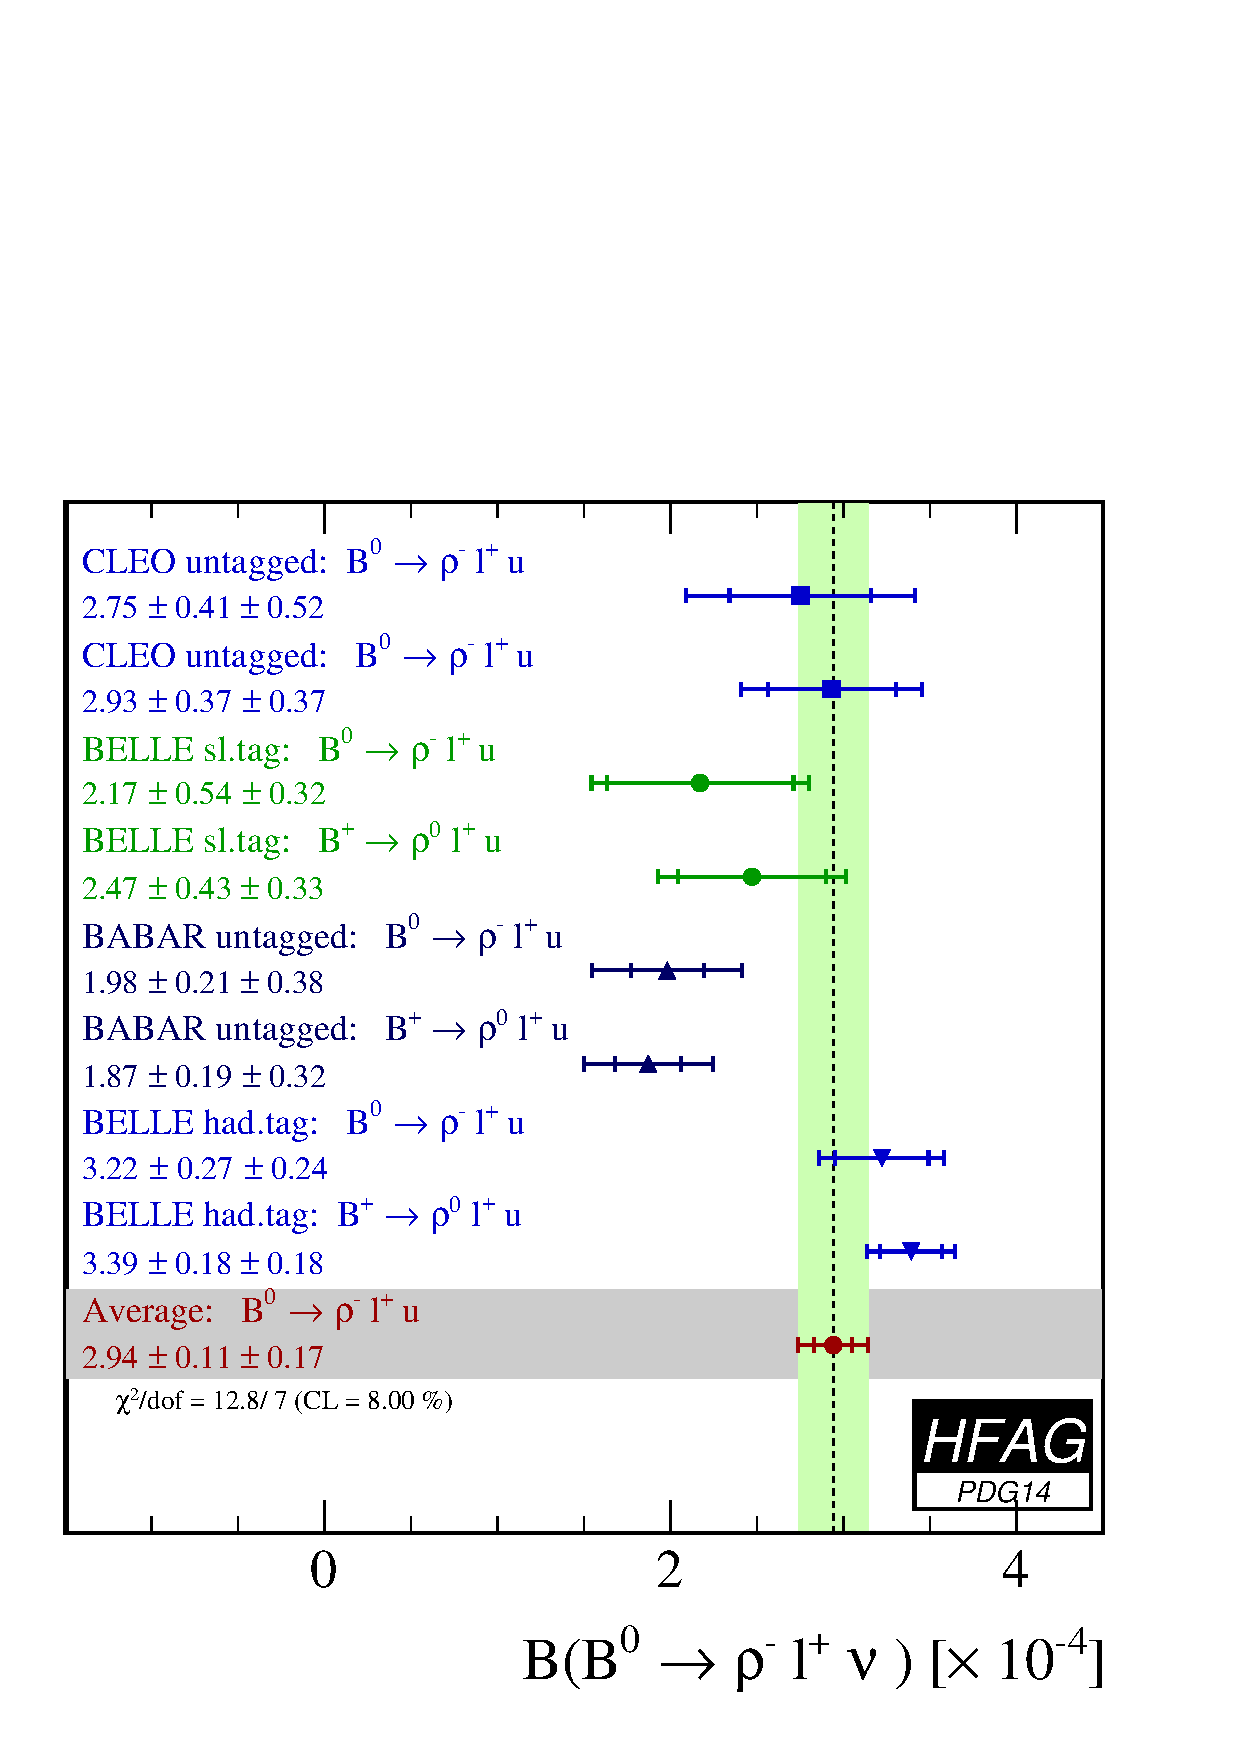
\includegraphics[width=8.0cm]{figures/slb/rholnu.pdf}}
   \put( 8.0,  0.0){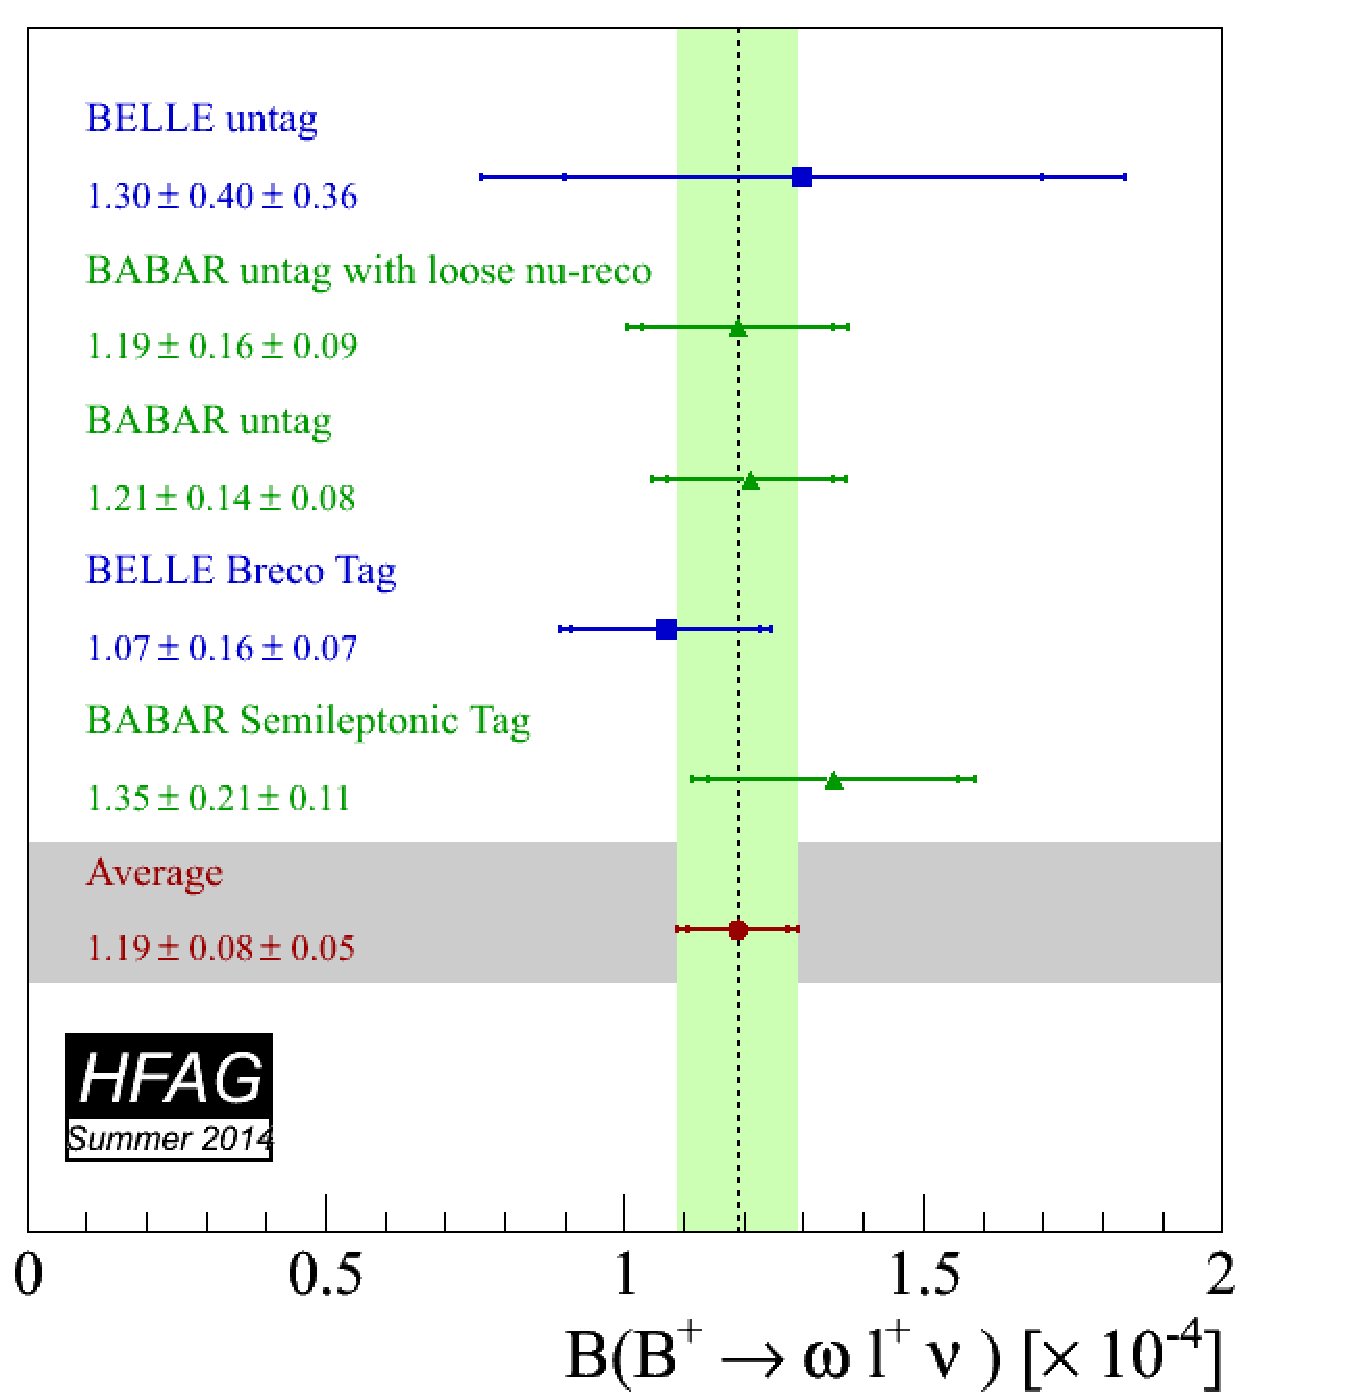
\includegraphics[width=8.0cm]{figures/slb/omegalnu.pdf}} 
   \put(  5.8,  7.5){{\large\bf a)}}  
   \put( 14.4,  7.5){{\large\bf b)}}
   \end{picture} \caption{
 (a) Summary of exclusive determinations of $\cbf(\Bb\to\rho\ell\nub)$ and their average. Measurements
 of $B^+ \to \rho^0\ell^+\nu$ branching fractions have been multiplied by $2\tau_{B^0}/\tau_{B^+}$ 
 in accordance with isospin symmetry.    
(b) Summary of exclusive determinations of $\cbf(\Bb\to\omega\ell\nub)$ and their average.
}
\label{fig:xulnu1}
\end{center}
\end{figure}

\begin{figure}[!ht]
 \begin{center}
  \unitlength1.0cm % coordinates in cm
  \begin{picture}(14.,8.0)  %ys(25.,6.)
   \put( -0.5,  0.0){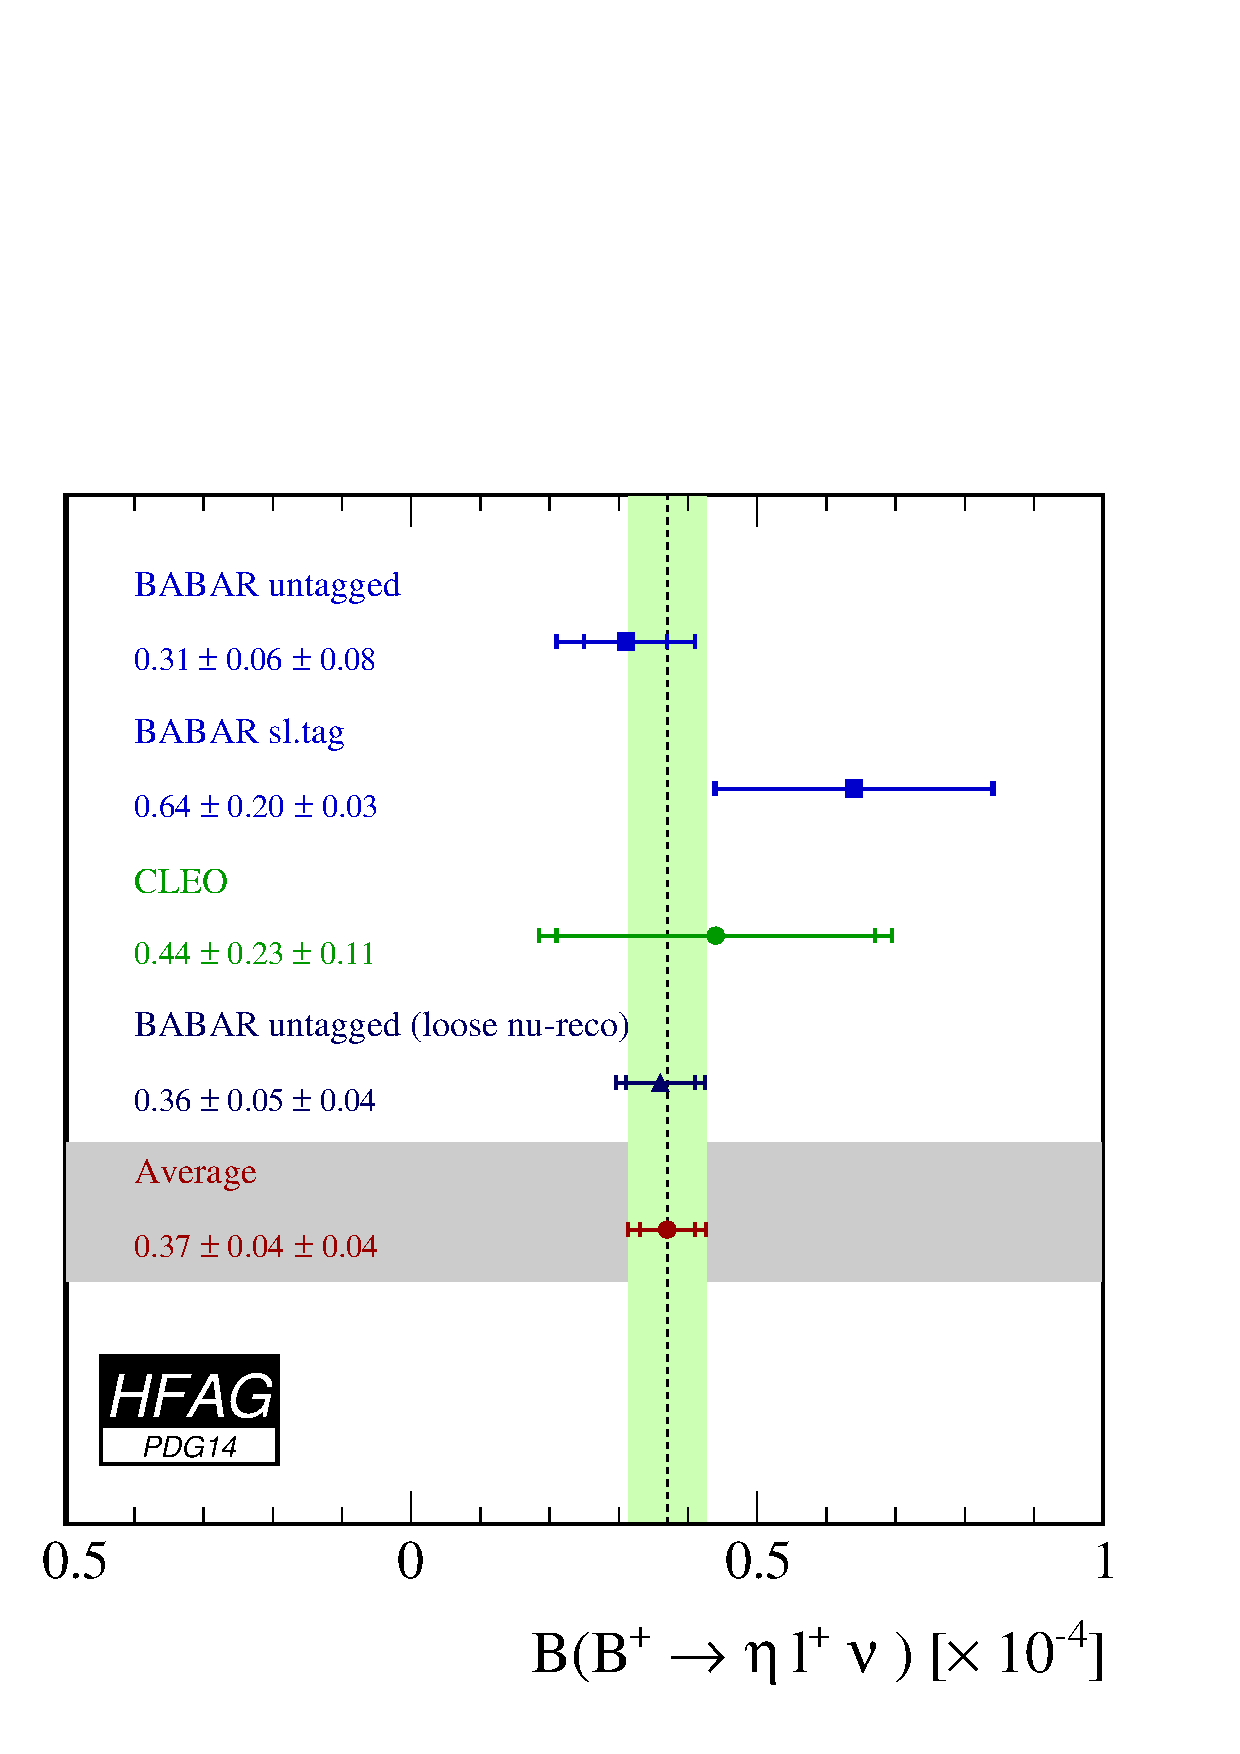
\includegraphics[width=8.0cm]{figures/slb/etalnu.pdf}}
   \put( 8.0,  0.0){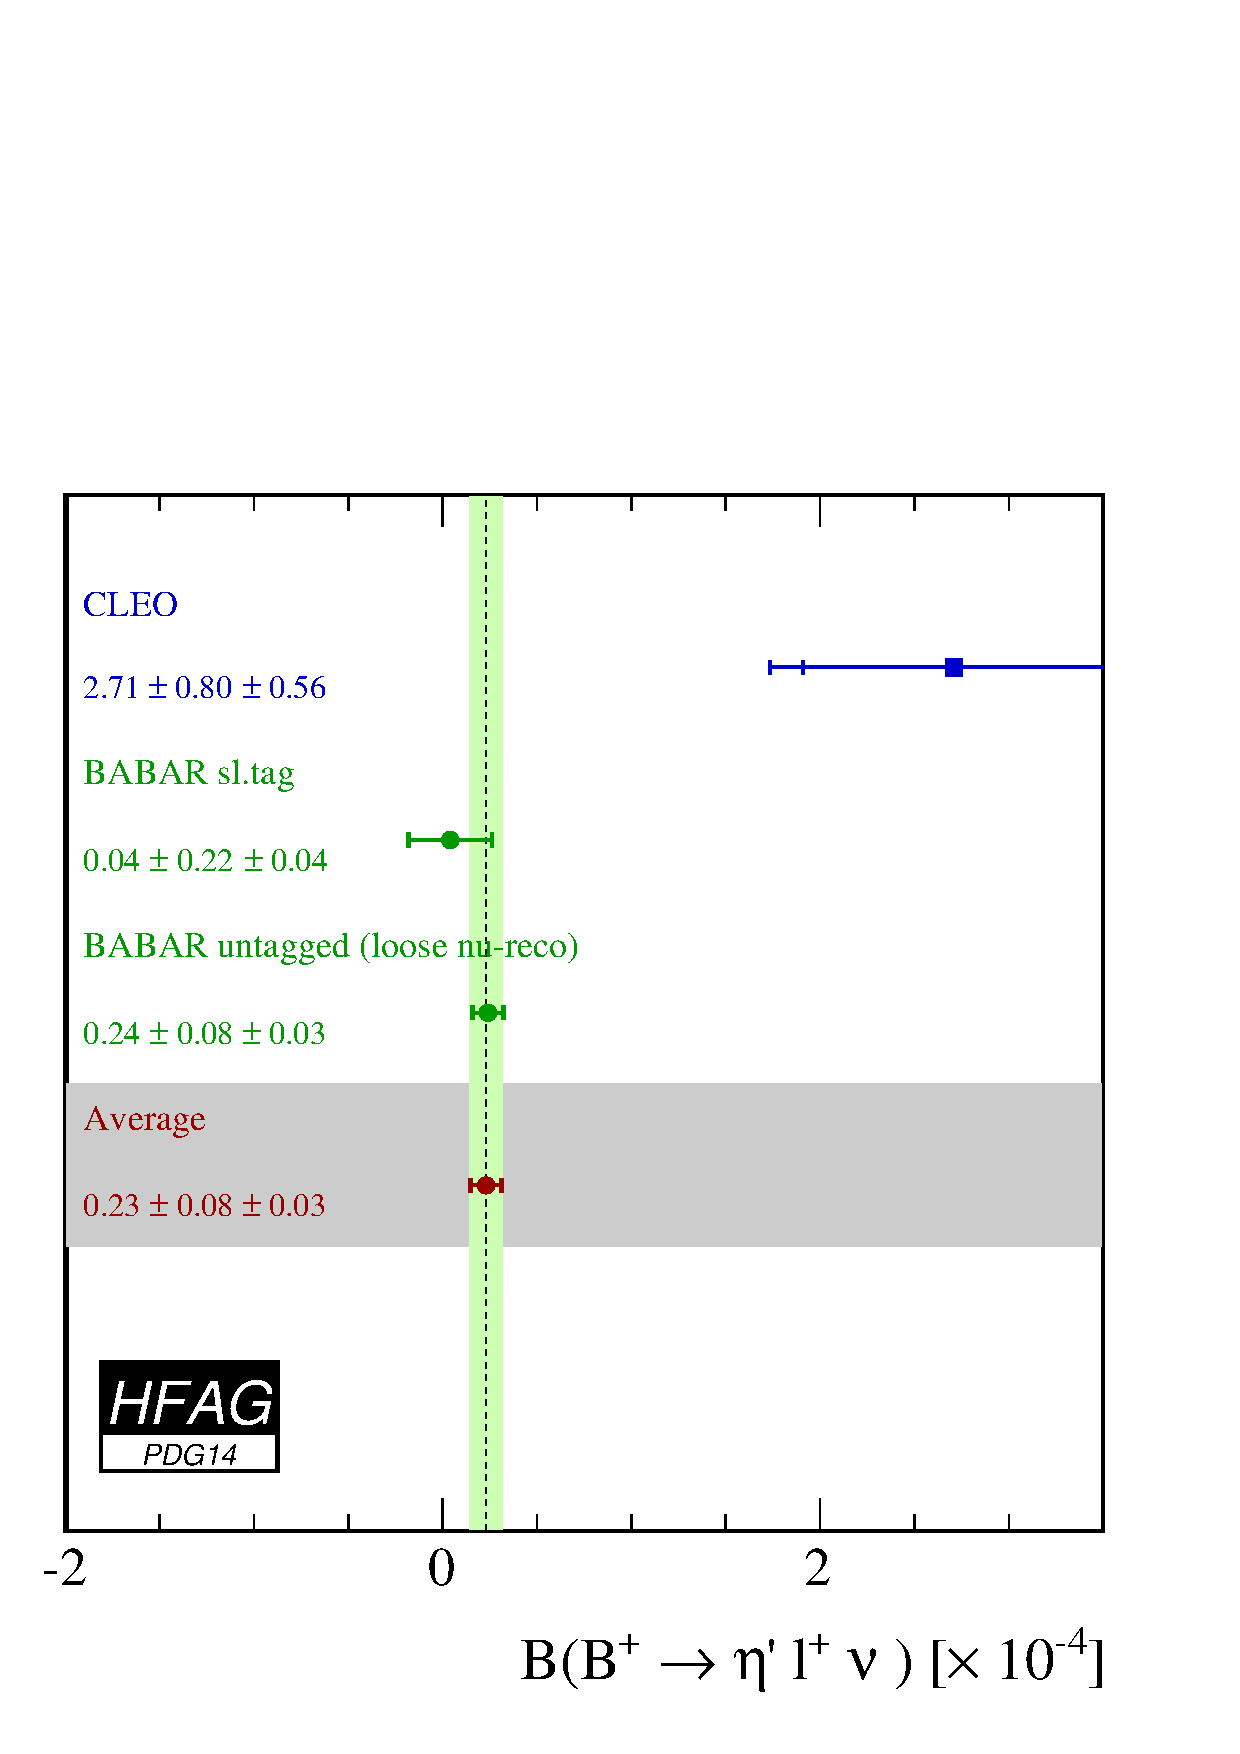
\includegraphics[width=8.0cm]{figures/slb/etaprimelnu.pdf}} 
   \put(  5.5,  7.3){{\large\bf a)}}     
   \put( 14.4,  7.3){{\large\bf b)}}
   
   \end{picture} \caption{
(a) Summary of exclusive determinations of $\cbf(\Bb\to\eta\ell\nub)$ and their average.
(b) Summary of exclusive determinations of $\cbf(\Bb\to\eta'\ell\nub)$ and their average.
}
\label{fig:xulnu2}
\end{center}
\end{figure}

%Branching fractions for other $\Bb\to X_u\ell\nub$ decays are given in
%Table~\ref{tab:xslother}. 
%\input{tables/slb/xslother.tex}

% ----------------------------------------------------------------------
